\chptr{Dinamica}
\marginpar{\minitoc}

\section{Recap}
\[ \overrightarrow{x} = \overrightarrow{x_0} + \overrightarrow{v}(t - t_0) \]
Semplificazioni in termini di variazioni, infinità.

\section{Leggi della dinamica}

Nella descrizione introduttiva del moto, non è stata analizzata alcuna causa del
fenomeno.

\subsection{La prima legge}

\vspace{8pt}
\begin{tcolorbox}[colback = red!30, colframe = red!30!black, title = {Prima legge della dinamica (legge di inerzia)}]
    Un corpo permane nel suo stato di \textit{quiete} o moto rettilineo uniforme
    finché non intervenga un \textit{agente esterno}.
\end{tcolorbox}
\vspace{5pt}

In altre parole, se nulla ``rompe le scatole'' al corpo, esso permanerà nel suo
stato di moto, naturalmente.

\vspace{8pt}
\begin{tcolorbox}[colback = yellow!30, colframe = yellow!30!black, title = {Sistema inerziale}]
    Sistema nel quale vale la prima legge della dinamica.
\end{tcolorbox}
\vspace{5pt}

\subsection{La seconda legge}
Quando l'agente esterno agisce sull'oggetto, l'effetto è un cambiamento nello
stato di moto di quell'oggetto. Ovvero, cambia la sua velocità. La variazione
della velocità nel tempo è chiamata \textbf{accelerazione}.

\[ \lim_{\Delta t \to 0} \frac{\Delta v}{\Delta t} = \frac{dv}{dt} = a \]

\vspace{8pt}
\begin{tcolorbox}[colback = red!30, colframe = red!30!black, title = {Seconda legge della dinamica}]
    \begin{align}
        \frac{|\overrightarrow{F}|}{|\overrightarrow{a}|} = \frac{F}{a} = m
    \end{align}
\end{tcolorbox}
\vspace{5pt}


Gli oggetti hanno inerzia, ovvero capacità di opporsi all'agire dell'agente
esterno. Questa capacità di opporsi è rappresentato da una quantità detta
massa (inerziale).

\subsection{Analisi dimensionale}
\[ [F] = [ma] = \left[m\cdot\frac{v}{t}\right] = \left[m\cdot\frac{l}{t^2}\right]  \]
\[ 1\text{ kg}\cdot\frac{\text{m}}{\text{s}^2} = \text{udm}\left[M\cdot\frac{L}{T^2}\right] = \text{udm}[F] = 1\text{ N} \]


\subsection{Molla e forza elastica}
\[ F \propto \Delta x \]

La forza che la molla esercita, essendo in opposizione alla direzione nella
quale la deformazione viene effettuata, corrisponde a:
\[ F_\textit{el} = -k\Delta x \]

\section{Forza agente sul moto}
Un blocco di massa $m = 10 \text{ kg}$ viaggia ad una velocità $v_i =
2 \text{ m/s}$. Una forza $F = 20 \text{ N}$ agisce sul blocco per
$T = 5 \text{ s}$. Quale velocità raggiungerà il blocco dopo $T$?.
Dopo $T$, la forza cessa di agire e il blocco viaggia a $v_f$ trovata
precedentemente. Includendo lo spazio percorso durante $T$ (e dunque il
tempo $T$), quanto tempo impiega il blocco a coprire $s_w = 2\text{ km}$
di distanza?

\begin{marginfigure}
    \centering
    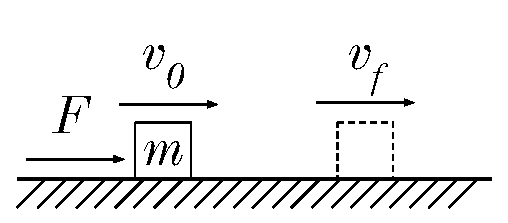
\includegraphics[width = \marginparwidth]{figures/scivola.pdf}
    \caption{Forza agente su una massa in moto}
\end{marginfigure}

Per rispondere al primo quesito, possiamo assumere un moto rettilineo
uniformemente accelerato durante l'intervallo $T$. Sappiamo che \[ a = \frac{F}{m} = \frac{dv}{dt} \]
Da cui possiamo esprimere la velocità in funzione del tempo (la velocità
iniziale la conosciamo già, ma assumiamo un tempo iniziale $t_0 = 0$):
\[ \frac{F}{m}dt = dv \to \int_{t_0}^{t}\frac{F}{m}dp = \int_{v_0}^{v}dw \to \frac{F}{m}\int_{0}^{t}dp = v - v_0 \to \frac{F}{m}t = v - v_0 \]
Dunque
\[ v(t) = v_0 + \frac{F}{m}t \]
Non ci manca che calcolare la velocità in corrispondenza di un $t_f = t_0 + \Delta t = 0 + T = T$:
\[ v(t_f) = v(T) = v_0 + \frac{F}{m}T \]

Nel secondo quesito, possiamo spezzare il problema in due parti: durante
l'azione della forza, la distanza percorsa ($s_a$) deve essere calcolata tenendo
conto del moto uniformemente accelerato, mentre nell'intervallo di tempo
successivo ($T_v$) il moto è semplicemente uniforme. Dalla seguente equazione,
possiamo ricavare $T_v$ ($T$ lo conosciamo già).
\[ s_w = s_a + s_v = s_a + v_fT_v = \int_{0}^{T}(v_0 + at)dp + v_fT_v = v_0T + \frac{1}{2}aT^2 + v_fT_v \]
Il tempo per percorrere $2\text{ km}$ è dunque:
\[ T_{2\text{ km}} = T + \frac{s_w - v_iT - \frac{F}{2m}T^2}{v_f} = T + \frac{s_w - v_iT - \frac{F}{2m}T^2}{v_i + \frac{F}{m}T} \]

\section{Lancio verso l'alto}
Si consideri la situazione mostrata in Figura \ref{lanciobasso}.
Durante la salita, l'oggetto rallenta a causa dell'accelerazione di gravità $g$.
Determiniamo la quota che l'oggetto raggiungerà.

\[ a = \frac{dv}{dt} \to dv = adt \to \int_{v_0}^{v}dw = \int_{t_0}^{t}adp \to v - v_0 = a\int_{t_0}^{t}dp \to v - v_0 = a(t - t_0) \]
Dunque
\[ v(t) = v_0 + a(t - t_0) = v_0 + at \]
Rallentando, si arriverà ad un istante $t_f$ nel quale l'oggetto avrà velocità
nulla:
\begin{marginfigure}
    \centering
    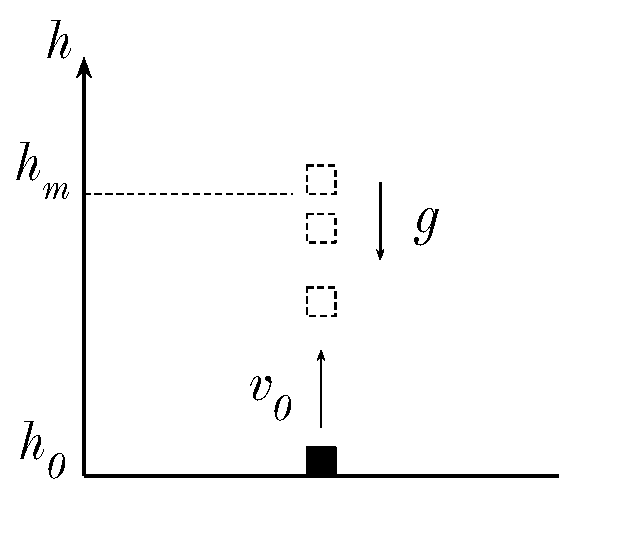
\includegraphics[width = \marginparwidth]{figures/greve.pdf}
    \caption{Lancio di un oggetto verso l'alto}
    \label{lanciobasso}
\end{marginfigure}
\[ v(t_f) = 0 \to v_0 + at_f = 0 \]
Non disponiamo tuttavia del tempo, ma possiamo avvalerci della legge oraria
che descrive la distanza percorsa:
\[ v(t) = \frac{dh}{dt} \to \int_{h_0}^{h}dk = \int_{t_0}^{t}v(t)dp \to h - h_0 = \int_{t_0}^{t}(v_0 + ap)dp \]
\[ h - h_0 = v_0\int_{t_0}^{t}dp + a\int_{t_0}^{t}pdp \to h - h_0 = v_0t + \frac12 at^2 \]
Da cui:
\[ h(t) = h_0 + v_0t + \frac12 at^2 = v_0t + \frac12 at^2 \]
Abbiamo quindi ottenuto la quota in funzione del tempo, che possiamo ricavare
dall'equazione $v_0 + at_f = 0 \to t_f = -\frac{v_0}{a}$.
\[ h(t_f) = v_0t_f + \frac12 at_{f}^2 =  -\frac{v_0^2}{a} + \frac{1}{2}a\frac{v_0^2}{a^2} = -\frac{v_0^2}{a} + \frac{v_0^2}{2a} = -\frac{v_0^2}{2a} \]
Sapendo che $a = -|g|$, la quota massima $h_m$ raggiunta è:
\[ h_m = \frac{v_0^2}{2|g|} \]

%%%%%%%%%%%%%%%%%%%%%%%%%%%%%%%%%%%%%%%%%%%%%%%%%%%%%%%%%%%%%%%%%

\subsection*{Spostamento}
\[ \Delta\overrightarrow{s} = \overrightarrow{s}_f - \overrightarrow{s}_i \]


\subsection{La terza legge}
\vspace{8pt}
\begin{tcolorbox}[colback = red!30, colframe = red!30!black, title = {Terza legge della dinamica}]

\end{tcolorbox}
\vspace{5pt}



\vspace{8pt}
\begin{tcolorbox}[colback = red!30, colframe = red!30!black, title = {Accelerazione centripeta nel moto circolare uniforme}]
\begin{align}
    a = \frac{v^2}{r} = \omega^2 r
\end{align}
\end{tcolorbox}
\vspace{5pt}


\section{Statica}
\[ \sum_{i = 1}^{N}\overrightarrow{F}_i = m\overrightarrow{a} \]
La somma nel membro di sinistra è detta \textit{risultante} ($\overrightarrow{R}$).
In quiete, non c'è accelerazione:
\[ \overrightarrow{R} = \overrightarrow{0} \]
Se la velocità è costante, possiamo parlare di problemi di quiete? Yes.

\subsection*{Esercizio}
$\overrightarrow{P} + \overrightarrow{T} = \overrightarrow{0} \Rightarrow -mg + T = 0 \Rightarrow T = mg$.

\begin{marginfigure}
    \centering
    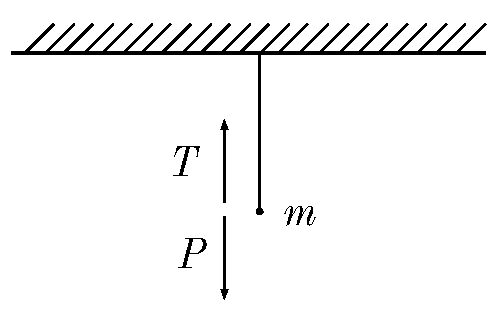
\includegraphics[width = \marginparwidth]{figures/statica.pdf}
    \caption{Massa appesa ad un filo}
    \label{filo}
\end{marginfigure}

\subsection*{Esercizio}
Come quello precedente ma con due corde che tengono $m$, inclinate di
tot gradi fissate al soffitto. Trovare la tensione su ciascun filo.




\section{Dinamica e moti armonici}
Tratteremo il moto armonico introducendo elementi di dinamica newtoniana,
studiando in particolare i cosiddetti \textit{oscillatori armonici}.
\vspace{8pt}
\begin{tcolorbox}[colback = yellow!30, colframe = yellow!30!black, title = {Oscillatore armonico}]
    Un oscillatore armonico è un oggetto su cui agisce una forza proporzionale,
    in modulo, allo spostamento dalla posizione di equilibrio e diretta in
    verso opposto rispetto a tale spostamento.
\end{tcolorbox}
\vspace{5pt}
Saranno due gli oscillatori armonici di nostro interesse: l'oscillatore a
molla e il pendolo semplice. Tuttavia, esistono numerosi esempi di oscillatori
armonici in natura, come uno snowboarder che compie evoluzioni in un half-pipe o
un atomo che vibra intorno al suo punto di equilibrio (con le dovute approssimazioni).



\subsection{Le equazioni del moto armonico}
\[ \theta(t) = A\sin(\omega t + \phi) = A\sin(\omega(t - t_0)) \]
\begin{itemize}
    \item $A$ ampiezza
    \item $\phi$ fase: $\phi = -\omega t_0$
\end{itemize}
\[ \frac{d^2\theta}{dt^2} = \frac{d}{dt}\frac{d\theta}{dt} = \frac{d}{dt}(A\omega\cos(\omega t + \phi)) = -\omega^2 A\sin(\omega t + \phi) = -\omega^2\theta \]
Sostituendo nell'equaione armonica funziona tutto.

\subsubsection{Interpretazione della pulsazione}
In tutte le equazioni dei moti armonici dominano le funzioni goniometriche.
Esse sono periodiche, ovvero esiste una quantità $T$ tale per cui $f(x + T) =
f(x)$ per ogni $x$ appartenente al dominio di $f$. In parole meno fredde,
dopo un certo \textit{periodo} la funzione si ripete, ciclicamente. Per seno
e coseno, il periodo corrisponde a $2\pi$ (infatti, vale per esempio $\sin(x+2\pi) =
\sin(x) \quad \forall x$).

Isoliamo la componente goniometrica delle equazioni armoniche, considerando
per esempio il seno e ignorando la fase $\phi$ (per il coseno il ragionamento
è analogo, mentre per $\phi$ possiamo risolvere il problema mediante trasformazioni).
Supponiamo di avere il periodo $T$, ovvero quel valore per cui la funzione ritorna
uguale a se stessa:
\[ \sin(\omega t) = \sin(\omega(t + T)) = \sin(\omega t + \omega T) \]
Sapendo che il periodo del seno è $2\pi$:
\[ \omega T = 2\pi \quad \therefore \quad \omega = \frac{2\pi}{T} \]
Possiamo dunque comprendere il significato della pulsazione $\omega$:
il suo valore è inversamente proporzionale al periodo $T$, ovvero la
pulsazione cresce al diminuire di $T$, e viceversa. Questo vuol dire
che $\omega$ fornisce un indice della ``rapidità'' con la quale le
oscillazioni di un moto armonico avvengono. Graficamente, $\omega$
comprime verso l'asse dell'ampiezza la funzione goniometrica quando il suo
valore cresce.

\subsection{L'oscillatore a molla}
Consideriamo un carrello di una rotaia a cuscino d'aria di massa $m$ attaccato
ad una molla di costante elastica $k$, indice della durezza della molla. Quando la molla si trova nella
posizione di equilibrio, cioè né estesa né compressa, il carrello rimane
fermo. Poniamo questa posizione come l'origine $x_o = 0$ di un asse delle
posizioni. Se il carrello viene spostato dall'equilibrio e portato a una
distanza $\overline{x}$ da tale posizione, la molla esercita una forza
elastica di \textit{richiamo} che, per la legge di Hooke, corrisponde a
\[ F = -k(x - x_o) = -kx \]
Il segno negativo indica appunto che si tratta di una forza di richiamo,
dunque opposta, nel suo verso, allo spostamento dalla posizione di equilibrio.
Possiamo applicare la seconda legge di newton:
\[ -kx = ma = m\frac{d}{dt}(v) = m\frac{d}{dt}\frac{d}{dt}(x) = m\frac{d^2x}{dt^2} \]
Da cui
\[ \frac{d^2x}{dt^2} + \frac{k}{m}x = 0 \]
Abbiamo mostrato che


$x(t) = A\sin(\omega t + \phi)$, $T = \frac{2\pi}{\omega} = 2\pi\sqrt{\frac{m}{k}}$.


\subsubsection*{Misurare dinamicamente $k$ di molle per ammortizzatori}
$m = 1500\text{ kg}$ (massa di una ruota per quattro).
\[ k = m_r\frac{4\pi^2}{T^2} = m\frac{\pi^2}{T^2} \simeq 1500\frac{10}{1\text{ s}}\text{ kg/s$^2$}\]
$T \simeq 1\text{ s}$.



\subsection{Il pendolo}
Quello del pendolo semplice è un sistema fisico descrivibile mediante
il modello del moto armonico. Un pendolo semplice è formato da una massa
$m$ appesa ad un filo o un'asta (idealmente inestensibili e di massa
trascurabile) con una certa lunghezza $l$. Il punto di equilibrio stabile del pendolo si trova
esattamente al di sotto del punto di sospensione. Di fatto, la posizione
a riposo corrisponde a quella illustrata nel sistema della Figura
\ref{filo}, dove è stato appunto mostrato che la risultante delle
forze agenti sulla massa appesa è nulla.

Supponiamo di spostare la massa dalla sua posizione di equilibrio,
formando un angolo $\theta$ tra il filo e la verticale. Sappiamo che
la massa può oscillare lungo un arco di circonferenza. Fissiamo un
sistema di riferimento solidale alla massa, con un asse coincidente con
la retta passante per il filo e l'altro ad esso perpendicolare, dunque
tangente all'arco. Scomponiamo dunque il peso della massa lungo questi
assi (perpendicolare e tangenziale)  e applichiamo la seconda legge della
dinamica:
\[ ma_t = P_t = -mg\sin\theta \]
\[ ma_n = - P_n + T + F_c = 0 \]
Notare che nella seconda equazione è presente anche la forza centripeta
$F_c$ derivante dal moto circolare, oltre la tensione. Concentriamoci
sull'accelerazione tangenziale nella prima equazione. Ricordando che gli
angoli sono in relazione con la lunghezza degli archi $a$ secondo
l'equazione $a = l\theta$:
\[ a_t = \frac{dv_t}{dt} = \frac{d}{dt}\left(\frac{ld\theta}{dt}\right) = l\frac{d^2\theta}{dt^2} \]
Dunque, riprendendo la primissima equazione riguardo la componente
tangenziale del peso, semplificando la massa:
\[ l\frac{d^2\theta}{dt^2} + g\sin\theta = 0 \]
Per rendere più semplice la trattazione del sistema fisico, supporremo
per ipotesi che $\theta\ll 1$ (in radianti), dunque ciò che calcoleremo
in seguito varrà solamente per piccole oscillazioni del pendolo.
\marginpar{
    \footnotesize
    %\hspace*{-0.5cm}
    \begin{tabular}{c|c|c}
        Prima                      & $\varepsilon\to0$ & Dopo\\
        \hline
        $\sin\varepsilon$          &                   & $\varepsilon$\\
        $\tan\varepsilon$          &                   & $\varepsilon$\\
        $\cos\varepsilon$          &                   & $1 - \frac{\varepsilon^2}{2}$\\
        $e^\varepsilon$            &                   & $1 + \varepsilon$\\
        $(1 + \varepsilon)^\alpha$ &                   & $1 + \alpha\varepsilon$
    \end{tabular}
}
Ricordando le proprietà delle serie di Taylor, possiamo approssimare
il seno nella precedente equazione, dividere per la lunghezza $l$ del
pendolo ottenendo
\[ \frac{d^2\theta}{dt^2} + \frac{g}{l}\theta = 0 \]
Diventa dunque evidente il motivo della semplificazione: abbiamo ottenuto
una relazione nella quale l'accelerazione (angolare) dipende proporzionalmente
dallo spostamento (angolare) con costante di proporzionalità negativa.
In altre parole, si tratta della descrizione di un moto armonico semplice
nella forma $\frac{d^2x}{dt^2} + \omega^2 x = 0$, dalla quale si deduce
che $\omega^2 = \frac{g}{l}$. Ma sapendo che $\omega^2 = (\frac{2\pi}{T})^2$
abbiamo modo di determinare il periodo di oscillazione del pendolo:
\begin{align}
    T = 2\pi\sqrt{\frac{l}{g}}
    \label{periodopendolo}
\end{align}


\subsubsection*{Isocronia delle piccole oscillazioni}
Come già aveva concluso Galileo nel 1583, il periodo di oscillazione
del pendolo, ristretta ad angoli ridotti a partire dalla posizione
di equilibrio, non dipende dall'ampiezza, come altri moti armonici.
Questo fatto è dimostrato dall'equazione precedentemente ottenuta
(Equazione \ref{periodopendolo}). Ciò che rende un pendolo diverso
dall'altro è la lunghezza del filo e ``il pianeta su cui si trova'',
intendendo l'accelerazione gravitazionale $g$. Mantenendo invariati
questi parametri, possiamo fissare una qualsiasi massa $m$ e caricare
il pendolo a nostro piacere (sempre entro i limiti di angoli ridotti),
ma $T$ non cambierà.

Il fatto che l'oscillazione non dipenda dalla massa fissata trova una
motivazione analoga a quella di una massa in caduta libera, dove
l'accelerazione è sempre la stessa. Masse ridotte si muovono più
facilmente per la loro piccola inerzia, ma tuttavia su di esse agisce
una forza altrettanto ridotta; d'altra parte, masse maggiori sono
sottoposte a forze gravitazionali maggiori, ma sono anche più difficili
da spostare.
Per giustificare intuitivamente l'indipendenza dall'ampiezza, è
sufficiente pensare che una maggiore ``carica'' è compensata da un
tragitto maggiore (l'arco di circonferenza descritto durante
l'oscillazione).

Possiamo dunque concludere che queste compensazioni sono il motivo
delle indipendenze osservabili nell'equazione \ref{periodopendolo}.

\subsubsection*{Analisi approfondita del moto di un pendolo}
Alla luce delle equazioni sul moto armonico semplice, definiamo la
velocità \textit{angolare} di una massa di un pendolo semplice:
\[ \nu = \frac{d\theta}{dt} = A\omega\cos(\omega t + \phi) \]
Ricordiamo che l'ampiezza $A$ corrisponde all'angolo massimo spazzato
durante l'oscillazione, quindi si tratta di una grandezza adimensionale,
seppur col significato di radianti. Per quanto riguarda l'accelerazione
angolare:
\[ \alpha = \frac{d\nu}{dt} = -A\omega^2\sin(\omega t + \phi) \]
Descriviamo $a$, l'arco di circonferenza descritto durante il moto,
sapendo che la lunghezza del filo è $l$:
\[ a = l\theta = lA\sin(\omega t + \phi) \]
Per quanto riguarda velocità tangenziale e accelerazione tangenziale:
\[ v_t = \frac{da}{dt} = \frac{d}{dt}(l\theta) = l\frac{d\theta}{dt} = l\nu = lA\omega\cos(\omega t + \phi) \]
\[ a_t = \frac{dv}{dt} = -lA\omega^2\sin(\omega t + \phi) \]


\subsubsection*{Tensione del filo di un pendolo semplice in funzione del tempo}
All'inizio di questa sottosezione, abbiamo analizzato le forze in gioco
distinguendo le componenti tangenziali e perpendicolari alla circonferenza
descritta dal pendolo. È ora di analizzare la componente perpendicolare,
la quale permette al pendolo di non distruggersi durante l'oscillazione.
Infatti, la massa è mantenuta nella sua traiettoria per mezzo della tensione
del filo, che si contrappone alla componente perpendicolare del peso della
massa appesa più la forza centripeta derivante dal moto circolare in atto.
La relazione tra i moduli di queste forze è dunque la seguente:
\[T = P_\perp + F_c = mg\cos\theta + ma_c = mg\cos\theta + m\frac{v_t^2}{l} \]
Data la variazione di $\theta$ e di $v_t$ durante l'oscillazione, segue
che la tensione dipende dal tempo. Approssimiamo l'equazione supponendo
$\theta\ll1$, possiamo utilizziare
l'equazione della velocità tangenziale ottenuta precedentemente:
\[ T(t) = mg\cos\theta(t) + mlA^2\omega^2\cos^2(\omega t + \phi) \]
Per via delle approssimazioni, possiamo semplificare anche la funzione coseno
dipendente da $\theta$, rimanendo con il termine $mg\theta(t)$. Avendo la
descrizione armonica $\theta(t) = A\sin(\omega t + \phi)$ otteniamo la funzione
della tensione di un pendolo per piccole oscillazioni:
\begin{align}
    T(t) = mg\left(1 - \frac{(a\sin(\omega t + \phi))^2}{2}\right) + mlA^2\omega^2\cos^2(\omega t + \phi)
\end{align}